\chapter{Hardware Implementation}

In the previous chapters each part of the system was explained, but with no information about how all these parts will work together to create the whole project, and that’s what this chapter is about. Communication, not surprisingly, is a role key in any V2V project either that communication is between vehicles and each other, objective of the project, or is between each module of the project.

\section{Embedded with JSON}
As explained previously the project constitutes of two main modules, vehicle unit, or embedded unit and server unit, to each its own goal in the case of embedded unit its purpose is to get various data about the vehicle and send it somehow to the Raspberry Pi, which allow the vehicle unit to communicate with the server therefore other vehicles. Since the goal is to send this data to other vehicles it was a must to package this data in a file, the type of file must be agreed upon, so other clients can extract the data from it successfully.

An interesting type of file that proved useful in this case is called JSON. JSON is a standard file format that uses human readable text to store and transmit data objects consisting of key value pairs, here is an example of JSON file that might be transferred between vehicles:



\begin{lstlisting}
{
	"speed": 60,
	"acceleration": 6
	"ip": 0.0.0.0
}

\end{lstlisting}

Of course data sent from the embedded unit isn’t in this format, so some processing must be done first to convert it to the agreed upon standard, fortunately working with strings is quite easy in Python it’s only a matter of simple string manipulation methods.\\

Data coming from embedded unit consists of two parts, data part and warning part the part that needs to be processed is the data one, a question mark is used to separate between these two parts, in each part there are key value pairs, A function named \textbf{write\_json\_file} is responsible to convert this format to JSON.

\clearpage
\begin{lstlisting}
import json
def write_json_file(file_name, formatted_string):
   """
   Writes a formatted string to a json file.
 
   Parameters
   ----------
   file_name : str
       The name of the file to write to.
   formatted_string : str
       The formatted string to write to the file.
   """
   json_object = {}
   for item in formatted_string.split("?"):
       if item[0] == "D":
           json_object["D"] = item.split(":")[1]
   with open(file_name, 'w') as f:
       f.write(json.dumps(json_object))
\end{lstlisting}

At first an empty dictionary, or object, is created to hold the key value pairs, then it loops over the string coming from STM and splits it over the delimiter, a question mark, to get the part that it’s concerned with, which is the data part, after that it adds each key value pair in this data to the empty dictionary, and finally it writes that dictionary to a json file.

\section{Embedded with server}

After all is said and done, a JSON file with data about the vehicle is created and waiting to be sent to the server which is responsible for broadcasting this file to other connected vehicles.\\

It was mentioned before that the component responsible for communication with the outer world is a Raspberry Pi as its purpose is to send and receive JSON files , but before explaining the mechanism by which that is achieved a problem is starting to rise, the Raspberry Pi is always receiving data from STM and at the same time it’s also receiving JSON files coming from the server so two different processes needs to be always running in order for the Raspberry Pi to achieve its main objective.\\

The two main processes are \textbf{uart\_handler} and \textbf{server\_handler},

\textbf{uart\_handler} is responsible for receiving data coming from STM, converting it to JSON format and sending JSON file to the server.
\clearpage
\begin{lstlisting}
def uart_handler():
   while True:
       receive_from_uart()
       print("Different file!")
       add_ip_address("files_to_be_sent/" + get_ip_address() + ".json")
       send_files(client, [get_ip_address() + ".json"])
\end{lstlisting}

Like it was mentioned before the Raspberry Pi needs to be always receiving and sending files to the STM, another function comes in handy here, \textbf{receive\_from\_uart} is the function that’s responsible for communicating with the STM.
\begin{lstlisting}
def receive_from_uart():
   ser = serial.Serial()
   ser.port = '/dev/ttyAMA0'
   ser.baudrate = 115200
   ser.timeout = 5
   ser.open()
 
   TXSize = 100
   RXSize = 100
   msgReceived = ''
 
   if (len(listdir("received_files")) > 0):
       msgSent = read_file(listdir("received_files")[0])
       msgSent = generate_formatted_string_from_json_string(msgSent)
       for i in range(len(msgSent), TXSize):
           msgSent += '!'
       ser.write(msgSent.encode())
 
   msgReceived = ser.read(RXSize)
   try:
       msgReceived.decode('utf-8')
       if(len(str(msgReceived)) > 3):
           write_json_file("files_to_be_sent/" + get_ip_address() + ".json",
                           str(msgReceived)[2:])
   except (UnicodeDecodeError, AttributeError):
       print("error")
       pass
   if msgReceived == b'\r':
       return
   msgReceived = ''

\end{lstlisting}
\clearpage
\textbf{receive\_from\_uart} does two things, check if there are any files ready to be sent to the STM and if there are it will first convert these JSON files to the format that’s understood by the STM and second it receives the data coming from the stm, convert it to a JSON file with the name of its ip.

Back to the main function that is \textbf{uart\_handler} after data from the STM is received and converted to the right format a key value pair is added to the JSON file that represents the ip of the Raspberry Pi, this key value pair helps the server to avoid sending the file back to the vehicle.

The second main process is called \textbf{server\textunderscore handler}:

\begin{lstlisting}
def server_handler():
   while True:
       receive_from_server(client_buffer)
\end{lstlisting}

Nothing fancy is happening here since most of the hard work is done in the function called \textbf{receive\textunderscore from\textunderscore server}:

\begin{lstlisting}
def receive_from_server(client_buffer):
   file_name = client_buffer.get_utf8()
   file_name = os.path.join('received_files', file_name)
   file_size = int(client_buffer.get_utf8())
 
   with open(file_name, 'wb') as f:
       remaining = file_size
       while remaining:
           chunk_size = BUFFER_SIZE if remaining >= BUFFER_SIZE else remaining
           print(chunk_size)
           chunk = client_buffer.get_bytes(chunk_size)
           if not chunk:
               break
           f.write(chunk)
           remaining -= len(chunk)
       if remaining:
           print('File incomplete.  Missing', remaining, 'bytes.')
       else:
           print('File received successfully.')
\end{lstlisting}

When the file is coming from the server, the first thing that’s sent is the file name, then the file size after that the file content will be sent over multiple chunks of constant size, each time a chunk is received the function checks to see if the file is complete or not.
\clearpage
These two main processes needs to be running in the same time:
\begin{lstlisting}
if __name__ == "__main__":
   p1 = Process(target=uart_handler)
   p1.start()
   p2 = Process(target=server_handler)
   p2.start()
   p1.join()
   p2.join()
\end{lstlisting}

Process is a method provided by multiprocessing library, so with these simple lines of code the Raspberry Pi functionality is complete.

\section{circuitry}
To simulate the project a prototype needed to prove the concept and to preform the proper
adjustments to test the data outputs, process it and to obtain
results.
The approach was to build two identical Robo-cars that can
represent the minimum V2V system, controlling the cars remotely.
\subsection{Motors}
A classic set of geared motor with a working voltage of 9V to 12V
equipped with the IR encoder rotary count disc made the basic motion system
\begin{figure}[h]
    \centering
    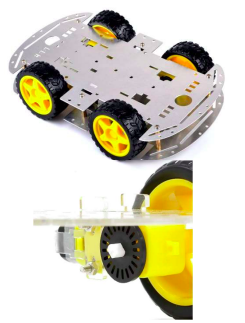
\includegraphics[scale=.5]{figures/9-3.png}
    \caption{Motors}
    \label{fig:motors}
\end{figure}
\subsection{Drivers}
to control the direction and speed of the motors, even the direction to preform different set of
motions start and stop the vehicle system needed a set of suitable motor drivers.
a motor driver of choice was the LM298D dual channel H—Bridge motor driver that was cheap yet
capable of doing the assigned task perfectly.
the driver have the function of controlling the speed using PWM signals and have 4 pins that control
the direction of each motor front or back separately.

\begin{figure}[h]
    \centering
    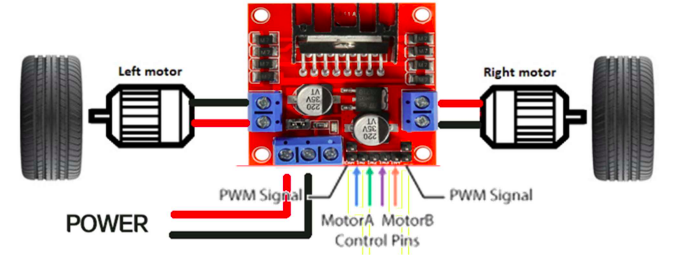
\includegraphics[scale=.5]{figures/9-4.png}
    \caption{Drivers}
\end{figure}


\subsection{Level Shifter}
The STM32 blue pill board uses logic 3.3V outputs while most component uses 5V logic high inputs so,
outputs of the STM32 needed to be shifted up to the 5V level hence using a MOSFET
level shifter solved the problem.

\begin{figure}[h]
    \centering
    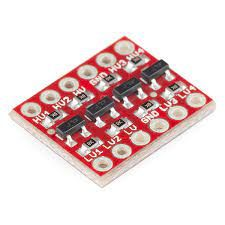
\includegraphics[scale=.5]{figures/9-5.jpeg}
    \caption{Level Shifter}
\end{figure}
\clearpage

\begin{figure}[h]
    \centering
    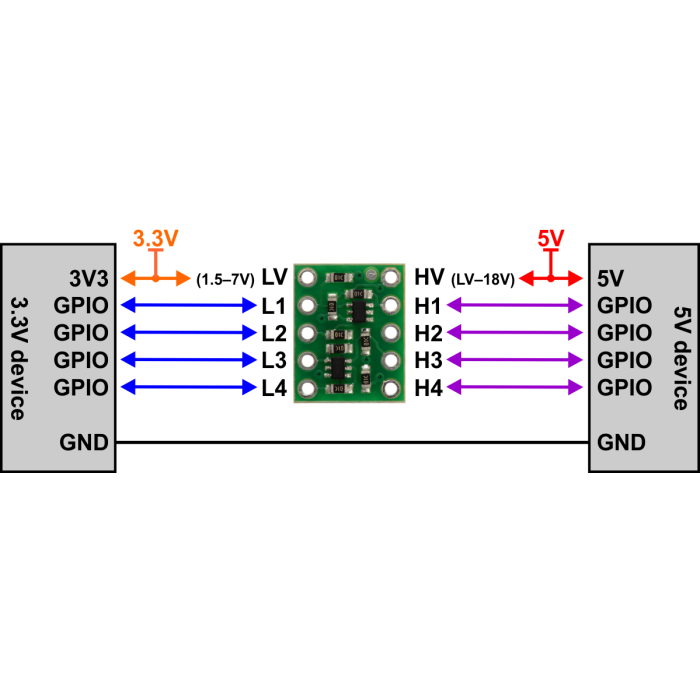
\includegraphics[scale=.5]{figures/9-6.png}
    \caption{Level Shifter Connection}
\end{figure}



\subsection{Bluetooth module}
To control the prototype car remotely, a Bluetooth module was used to receive control signal, using a Bluetooth based remote that can easily found or built –
 even a smart phone considered one – controlling the
car became a simple task.

\begin{figure}[h]
    \centering
    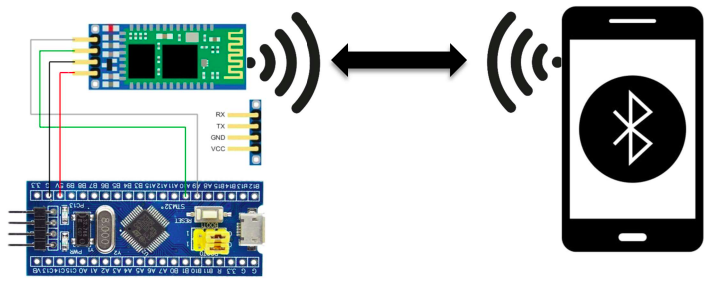
\includegraphics[scale=.3]{figures/9-7.png}
    \caption{Bluetooth Module Connection}
\end{figure}

\clearpage

\subsection{CAN Bus System}
Using CAN protocol which is an industrial standard needed to build its hardware system that consisted of a CAN controller, CAN module and CAN transceiver.

\begin{itemize}
    \item CAN Controller: Hardware wise CAN controller interface task was easy one as it’s already on the stm32-bluepill development board only needed to identify and connect with it’s pins.
    \item CAN Transceiver: CAN TRANSCEIVER used to send and receive CAN signal controlled by the STM 32 controller.
The TRANSCEIVER needed to be designed as it wasn’t found as a module in the local market so starting up with the tja1051t IC the
following circuit was made.
\begin{figure}[h]
    \centering
    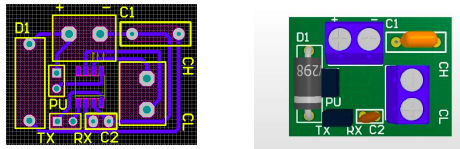
\includegraphics[scale=.5]{figures/9-8.png}
    \caption{CAN Transceiver PCB}
\end{figure}

    \item CAN Module: CAN module used to receive the CAN signal in devices we need to control if the
CAN protocol is not hardware implemented on it already.
The module used is MCP-2515.
    \begin{figure}[h]
    \centering
    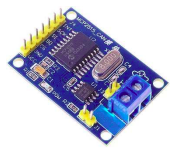
\includegraphics[scale=.6]{figures/9-9.png}
    \caption{CAN Module PCB}
\end{figure}
\end{itemize}

\section{Prototype}
First, the prototypes must be moving to be able to use them in V2X application by using four dc motors, two L298D motor drivers and one STM32F103C8T6 micro-controller for each prototype (car chassis). Then each assembly car is needed to be integrated with the micro-controller to be able to control it in a wireless method by Bluetooth. After that, Interaction between the assemble car and the project is implemented. Finally, the project is copied into the second assemble car and tests have to be done with the server.\\
In this section, previous steps will be discussed individually.

\subsection{Hardware Drivers}

The L298 is an integrated monolithic circuit in a 15- lead Multiwatt and PowerSO20 packages. It is a high voltage, a high current dual full-bridge driver designed to accept standard TTL logic levels and drive inductive loads such as relays, solenoids, and DC and stepping motors. Two enable inputs are provided to enable or disable the device independently of the input signals. The emitters of the lower transistors of each bridge are connected together and the corresponding external terminal can be used for the connection of an external sensing resistor. An additional supply input is provided so that the logic works at a lower voltage.

\begin{figure}[h]
    \centering
    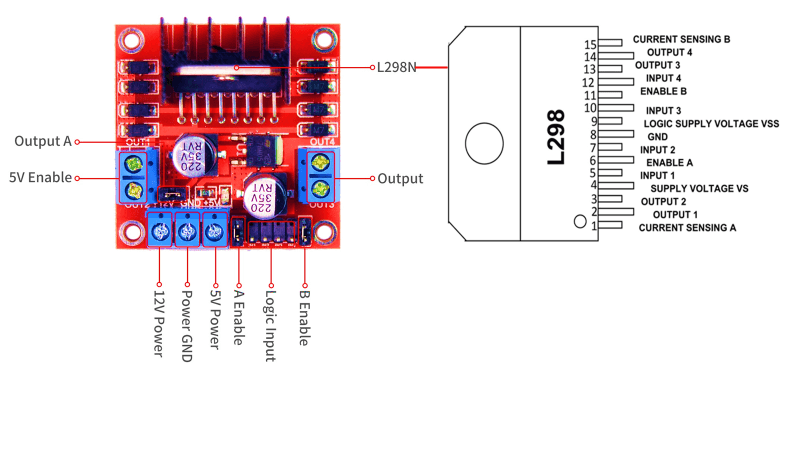
\includegraphics[scale=.4]{figures/9-10.png}
    \caption{L298D Motor Drivers}
\end{figure}

\begin{figure}[h]
    \centering
    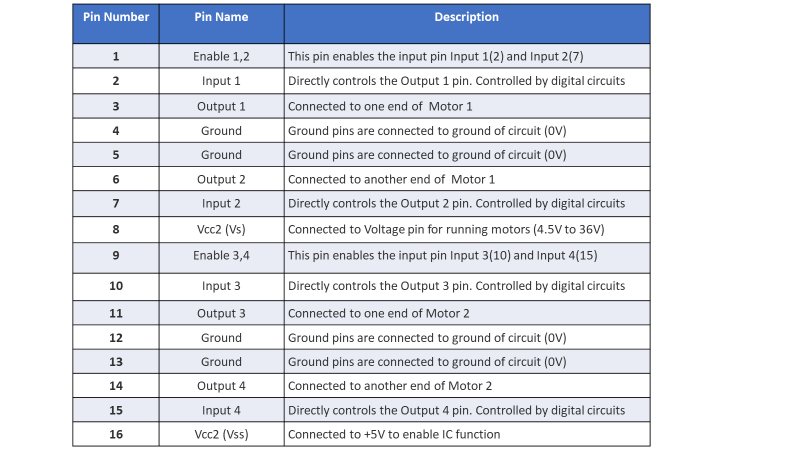
\includegraphics[scale=.5]{figures/9-11.png}
    \caption{L298D Motor Driver Pins}
\end{figure}
\newpage
The assembly car has two floors, Drivers are put in the lower floor as shown in figure \ref{fig:hardware-driver-cars}.

\begin{figure}[h]
    \centering
    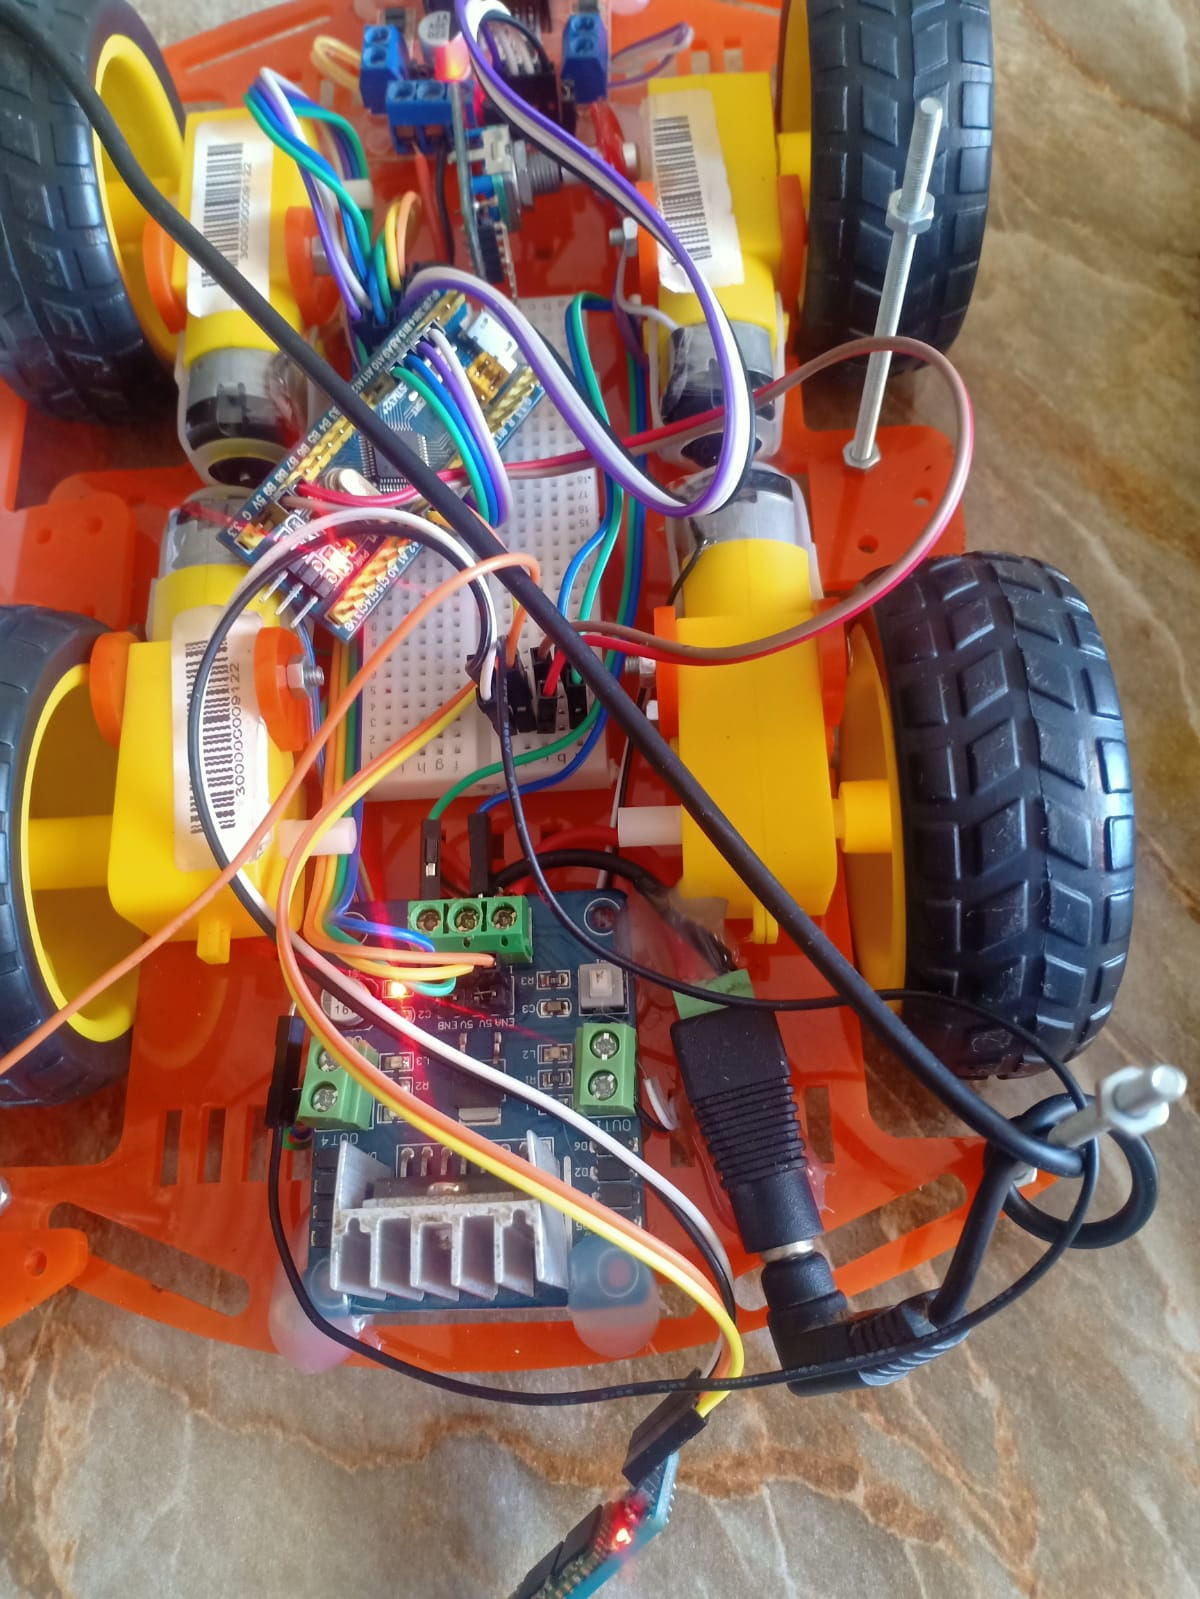
\includegraphics[width=.8\textwidth]{figures/9_13.jpg}
    \caption{Hardware Connection of Drivers in the assembly car}
    \label{fig:hardware-driver-cars}
\end{figure}

\subsubsection{Code Configuration}
Drivers need to generate a timer signal for controlling the moving, so in STM the timer is enabled with two channels; each channel in the PWM mode as shown in figure \ref{fig:stm-config}.
\newpage
\begin{figure}[h]
    \centering
    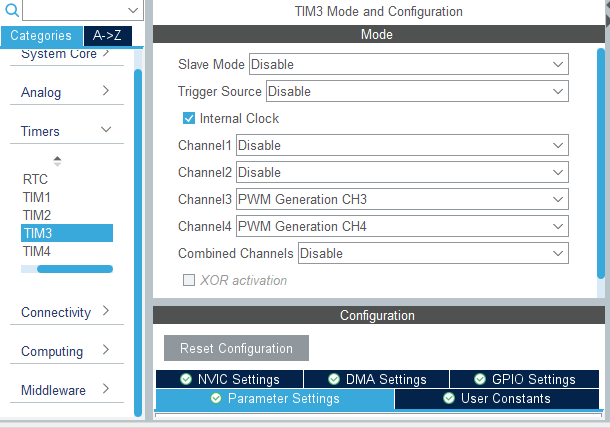
\includegraphics[width=.8\textwidth]{figures/9_14.PNG}
    \caption{STM configuration for Hardware Drivers}
    \label{fig:stm-config}
\end{figure}
Using the timer configuration, moving direction functions are implemented, for each direction there is a function to control it and it is called according to the wireless control. This will be discussed in next sub-section.
\\ \textbf{The implemented functions are:}
\begin{lstlisting}
void Left_Forward(void);
void Right_Forward(void);

void Left_Backward(void);
void Right_Backward(void);

void Left_Stop(void);
void Right_Stop(void);

void Forward(void);
void Backward(void);
void Stop(void);
void Left_Rot(void);
void Right_Rot(void);
void Left_Turn(void);
void Right_Turn(void);

void Speed_Up(void);
void Speed_Down(void);

void Fixed_Speed(void);
\end{lstlisting}
\subsection{Bluetooth Control}
In this subsection the remote control will be discussed and the code that was written to control the car. As said before the Bluetooth module is connected with a Mobile phone to share some data, then it can be connected with a micro-controller by UART to transmit this data to it. The same happened here, Bluetooth module is connected with a mobile phone to get a data from an Android software program called "Bluetooth RC Controller" as shown in figure \ref{fig:rc-bt}.

\begin{figure}[h]
    \centering
    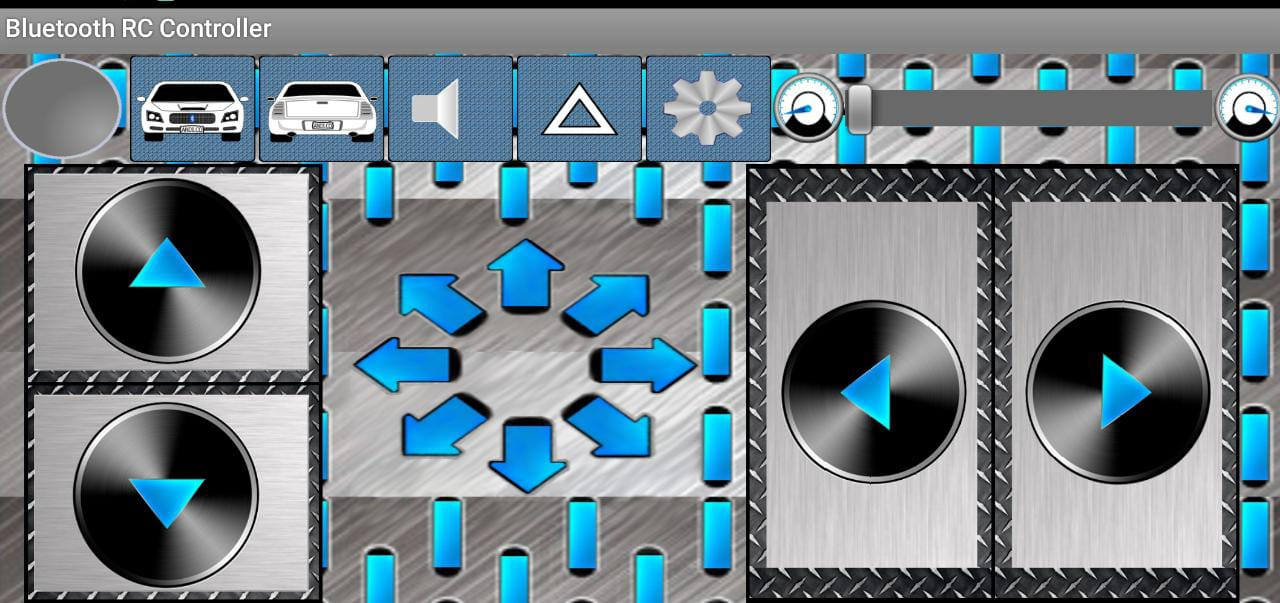
\includegraphics[width=.8\textwidth]{figures/9_15.jpg}
    \caption{RC Bluetooth Controller Software Application}
    \label{fig:rc-bt}
\end{figure}

while pressing on some button, it sends a specific character for Bluetooth module and then it is checked and compared using switch case statement in STM.

\subsubsection{Main function code: }
\begin{lstlisting}
int main(void)
{
	/* USER CODE BEGIN 1 */

	/* USER CODE END 1 */

	/* MCU Configuration--------------------------------------------------------*/

	/* Reset of all peripherals, Initializes the Flash interface and the Systick. */
	HAL_Init();

	/* USER CODE BEGIN Init */

	/* USER CODE END Init */

	/* Configure the system clock */
	SystemClock_Config();

	/* USER CODE BEGIN SysInit */

	/* USER CODE END SysInit */

	/* Initialize all configured peripherals */
	MX_GPIO_Init();
	MX_TIM3_Init();
	MX_USART2_UART_Init();
	/* USER CODE BEGIN 2 */
	HAL_TIM_PWM_Start(&htim3, TIM_CHANNEL_3);
	HAL_TIM_PWM_Start(&htim3, TIM_CHANNEL_4);
	/* USER CODE END 2 */

	/* Infiniteloop */
	/* USER CODE BEGIN WHILE */
	while (1)
	{
		/* USER CODE END WHILE */

		/* USER CODE BEGIN 3 */


		HAL_UART_Receive(&huart2, &CTRL, 1, HAL_MAX_DELAY);
		switch (CTRL)
		{
		case 'F':
			Forward();
			break;

		case 'B':
			Backward();
			break;

		case 'S':
			Stop();
			break;

		case 'L':
			Left_Rot();
			break;

		case 'R':
			Right_Rot();
			break;

		case 'G':
			Left_Turn();
			break;

		case 'I':
			Right_Turn();
			break;

		case 'U':
			Speed_Up();
			sprintf(MSG,"%d\n",Speed);
			HAL_UART_Transmit(&huart2, MSG, 4, HAL_MAX_DELAY);
			break;

		case 'D':
			Speed_Down();
			sprintf(MSG,"%d\n",Speed);
			HAL_UART_Transmit(&huart2, MSG, 4, HAL_MAX_DELAY);
			break;
		}
	}
	/* USER CODE END 3 */
}
\end{lstlisting}

\begin{wrapfigure}{r}{5cm}
    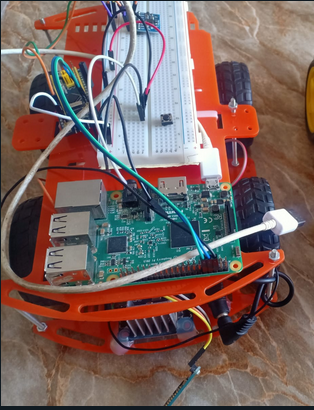
\includegraphics[width=0.5\textwidth]{figures/9_16.PNG}
    \caption{Complete assembly car design}
    \label{fig:complete-assembly}
\end{wrapfigure}
\subsection{Integration With The Project}
After successful remote control, the project was inserted to the assembly car, as said before the assembly car consists of two floors, the project is inserted on the upper floor as shown in figure \ref{fig:complete-assembly}.

\subsection{Project Copying}
After ensuring that all sensors work properly, the project has to be be copied on another assembly car to test between them and make them communicate through the server. Testing the two cars is done by making them move in which they will make an accident and it is expected that the two cars send a warning to be displayed. \\

\textbf{Finally, the basic structure for V2V is implemented and the project is excitedly ready for the applications. } 